

\par In order to achieve the ability to predict objects and scenes 
from FMRI images, a predictive model is required. The project was thus 
divided into a few main stages for independent preprocessing of the 
movie description and FMRI images, model building, and prediction
testing.

\centerline{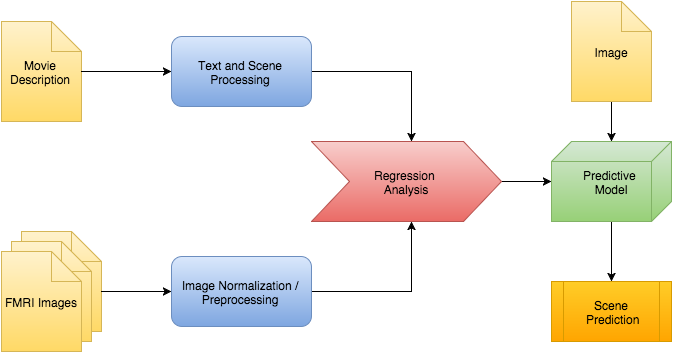
\includegraphics[width=.9\linewidth]{processflow}}

\subsection{Text Preprocessing}
\par As the movie description as provided was in German, we first used Google
Translate to translate the description to English before proceeding with 
any further processing. Though there may be translational errors, it was decided
that it was best to transform the original descriptions (versus using other english descriptions) to maintain the original timestamps from the researchers
to have optimal alignment between the description and FMRI data.

\par Due to grammatical differences, we decided to
 only keep nouns and verbs, and discarded the adjectives and other words including
 stopwords, which are commonly used words with little meaning or determinable context (e.g. 'and', 'to', 'him'). A publicly available list of stopwords from Princeton University was used for this task. 

 \par Of the words that remained, a WordNet dictionary was built.

 \centerline{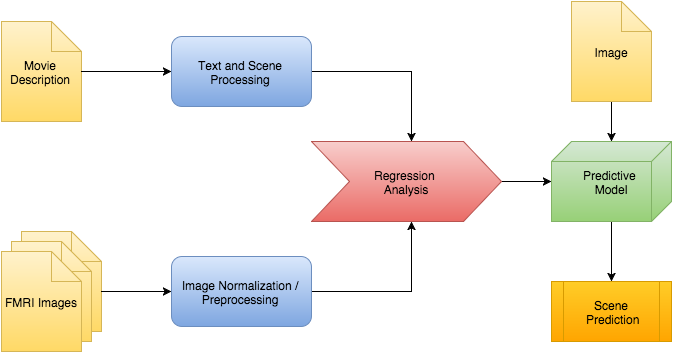
\includegraphics[width=.9\linewidth]{processflow}}

\subsection{FMRI Preprocessing}

\subsection{Regression Analysis}

\subsection{Predictive Testing}

